\documentclass{article}
\usepackage[utf8]{inputenc}
\usepackage{graphicx}
\usepackage{amsmath}
\usepackage{amsfonts}
\usepackage{amssymb}
\usepackage{makeidx}
\usepackage{graphicx}
\usepackage{lmodern}
\usepackage{verbatim}
\usepackage{multirow}
\usepackage{url}
\usepackage{hyperref}
\usepackage{float}
\usepackage[left=2.5cm,right=2.5cm,top=2.5cm,bottom=2.5cm]{geometry}
\usepackage{listings}
\usepackage{xcolor}
\definecolor{mygreen}{rgb}{0,0.6,0}
\definecolor{mygray}{rgb}{0.5,0.5,0.5}
\definecolor{mymauve}{rgb}{0.58,0,0.82}
\definecolor{myorange}{rgb}{1,0.64,0}
\def\groupe{Groupe C}
\def\PA{\begin{small}Teaching assistants:\end{small} Christophe Limbrée \begin{small}(Project Leader)\end{small} \& Emery Kouassi Assogba}
\def\Prof{\begin{small}Professor:\end{small} Dr Sébastien Combéfis}
\def\Client{\begin{small}Client:\end{small} Victor de Beco}

\lstdefinestyle{customc}{
  belowcaptionskip=1\baselineskip,
  breaklines=true,
  frame=ltrb,
  numbers=left,
  tabsize=3,
  escapeinside={\%*}{*)},
  xleftmargin=\parindent,
  language=Matlab,
  showstringspaces=false,
  basicstyle=\footnotesize\ttfamily,
  keywordstyle=\bfseries\color{blue},
  commentstyle=\itfshape\color{mygreen},
  identifierstyle=\color{black},
  stringstyle=\color{myorange},
  literate={á}{{\'a}}1 {ã}{{\~a}}1 {é}{{\'e}}1 {à}{{\`a}}1 {â}{{\^a}}1
}
\lstset{escapechar=@,style=customc}


%============================================================
% Page de garde
%============================================================
\makeatletter
\def\thickhrulefill{\leavevmode \leaders \hrule height 1pt\hfill \kern \z@}
\renewcommand{\maketitle}{\begin{titlepage}%
    \let\footnotesize\small
    \let\footnoterule\relax
    \parindent \z@
    \reset@font
    \null\vfil
    \hrule height 4pt
    \vskip 10\p@
    \begin{centering}
      \Huge
      \strut \@title \par
    \end{centering}
    \vskip 5\p@
    \begin{flushleft}
        \Large
        \strut \Prof \par
        \struct \PA \par
        \strut \Client \par
    \end{flushleft}
      \vskip 30\p@
    \begin{flushright}
      \Large
      \strut \groupe
    \end{flushright}
    \begin{flushright}
        \Large
        \strut \@author
    \end{flushright}
    \vskip 5\p@
    \hrule height 4pt
    \begin{flushright}
    \@date
    \end{flushright}
    \vskip 60\p@
    \vfil\null
  \end{titlepage}%
  \setcounter{footnote}{0}%
  \reset@font
}

\makeatother

\title{SEProject: Guide du programmeur}
\author{\begin{small}
\begin{tabular}{cccc}
Mokaddem Sami \qquad & Heymans Pierre \qquad & Francotte Florian & Pierre-Yves Dehon \\
Rollin Antoine \qquad & Marin Alicia \qquad & Murhububa Serge \\
\end{tabular}\end{small}
}
\date{\today}

\begin{document}

\maketitle

\section{Introduction}

In this guide, we'll explain the architecture of the website to make it understandable and modifiable by the client's programmer.

\section{Architecture globale}

L'architecture du site web est découpée en trois grande partie

\begin{itemize}
\item[$\bullet$] La page d'accueil est dans le dossier 'src'
\item[$\bullet$] Les formulaires d'inscription sont dans 'src/inscription'
\item[$\bullet$] L'interface staff est dans 'src/staff'
\end{itemize}\\

Langages utilisés
\begin{itemize}
\item[$\bullet$] Côté Client: \begin{itemize}
        \item[$\bullet$] HTML
        \item[$\bullet$] CSS
        \item[$\bullet$] Javascript
    \end{itemize}
\item[$\bullet$] Côté Serveur: \begin{itemize}
        \item[$\bullet$] PHP
        \item[$\bullet$] MySQL
    \end{itemize}
\end{itemize}\\

Framework utilisés
\begin{itemize}
\item[$\bullet$] CSS: \begin{itemize}
        \item[$\bullet$] Bootstrap
        \item[$\bullet$] Font-Awesome
    \end{itemize}
\item[$\bullet$] JS: \begin{itemize}
        \item[$\bullet$] Bootstrap
        \item[$\bullet$] Datatable
        \item[$\bullet$] jquery
    \end{itemize}
\end{itemize}\\


\begin{figure}[H]
\centering
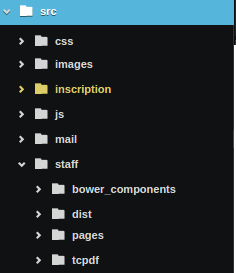
\includegraphics[scale=0.7]{Structure.png}
\caption{Arborescence de l'application}
\end{figure}


\section{Home page}
The home page is directly located in the directory 'src' and corresponds to the file 'src/index.php'.

\begin{itemize}
\item[$\bullet$] Link : src/index.php
\item[$\bullet$] Style : 'src/css'
\item[$\bullet$] JS : 'src/js'
\item[$\bullet$] Images 'src/images'
\end{itemize}

The framework CSS used is Twitter Bootstrap (bootstrap.min.css)\\
We also used a template for the page, style.css.
Our CSS is monStyle.css\\
\begin{figure}[H]
\centering
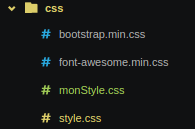
\includegraphics[scale=1]{CSSAccueil.png}
\caption{Styles used for the home user page}
\end{figure}

\\
The framework javascript used are Twitter Bootstrap and JQuery.\\
The template that we used provide a html5hiv.js and jqBootstrapValidation.js field verification of for forms.\\
And script.js for the design.\\
\begin{figure}[H]
\centering
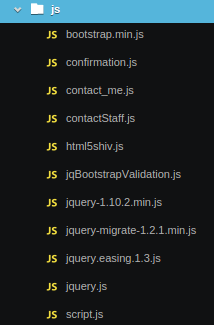
\includegraphics[scale=1]{JSAccueil.png}
\caption{Scripts used in the user home page}
\end{figure}

The files contact\_me.js, contactStaff.js are the function to be able to send mail through the home page.
\begin{figure}[H]
\centering
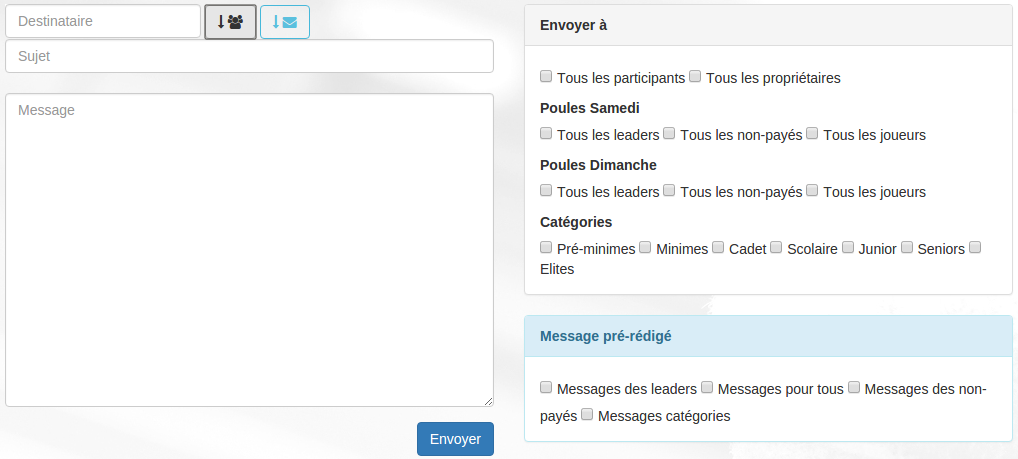
\includegraphics[scale=0.6]{mailAccueil.png}
\caption{Interface to contact the staff}
\end{figure}

\section{Registration Player \& Owner}

The registers forms for players and owners are located in the directory 'src/inscription'. Those are the forms that visitor will use to register.
The register form for player correspond to the file 'src/inscription/index.php'.\\
The register form for owner correspond to the file 'src/inscription/inscription-owner.php'.\\

\begin{figure}[H]
\centering
\includegraphics[scale=0,7]{arboInsccription.png}
\caption{Directory tree for registration, user side}
\end{figure}


\section{Staff Interface}

\subsection{Presentation}

\begin{itemize}
\item[$\bullet$] Link : src/staff/pages
\item[$\bullet$] Librairies/Dependences : src/staff/bower\_components
\item[$\bullet$] Style : 'src/staff/dist/css'
\item[$\bullet$] JS : 'src/staff/dist/js'
\item[$\bullet$] Tool for PDF generating : 'src/staff/tcpdf'
\end{itemize}

The librairies Twitter Bootstrap, Font-Awesome, JQuery and datatable have been essentially used.
Our personalised styles are in 'dist/'

\subsection{Addition, Edition and List}

First, the PHP files which are located in the directory \textit{src/staff/pages/} correspond to the displayed page in the application. This folder contain in fact every forms of addition, edition of entities (player, owner, court, match, ...). They are represented with PHP files. The edition forms are characterized by the word 'edit' in the beginning of the file whereas addition form are simply indicated by the name of the entity which correspond to. For instance, the file 'court.php' correspond to the add form of court, and the file 'edit-court.php' correspond to the edition form of a court. \\
% Premièrement, les fichiers php se trouvant dans le dossier \textit{src/staff/pages/} correspondent aux pages affichées dans l'application. Ce dossier contient en fait tous les formulaires d'ajout et d'édition des entités (joueur, propriétaire, terrain, match, …). Ils sont représentés par des fichier PHP. Les formulaires d'édition sont caractérisés par le mot 'edit' en début de nom de fichier alors que les formulaires d'ajout sont simplement désignés par le nom de l'entité qui leur correspond. Par exemple, le fichier 'court.php' correspond au formulaire d'ajout un terrain, et le fichier 'edit-court.php' correspond au formulaire d'édition d'un terrain. \\
Then, the folder \textit{src/staff/pages/html} contain the file 'header.php' which correspond to navigation bar visible on the left in each pages of the staff interface.
% Ensuite, le dossier \textit{src/staff/pages/html} contient un fichier 'header.php' qui correspond à l'en-tête visible sur toutes les pages de l'interface Staff, ce que nous appellons la "barre de navigation". \\
Plus, the files located in the folder \textit{src/staff/pages/php} will be called with get/post method during every interaction with the database, for instance during the validation form. The additions function are located in files which the name starts by 'add'. Deletion function are located in the files which the name starts by 'delete'. \\
%Enfin, les fichiers se trouvant dans le dossier \textit{src/staff/pages/php} seront appelés par des methodes get/post lors de toutes interaction avec la base de donnée, par exemple lors de la validation d'un formulaire. Les fonctions d'ajout sont situées dans les fichiers dont le nom commence par 'add'. Les fonctions de suppression sont situées dans les fichiers dont le nom commence par 'delete'. \\
Finally, the files inc of \textit{src/staff/pages/php/inc} contain most of function used in \textit{src/staff/pages/php}, in order to not overcharge the code those files. Edition function are located in the files wich the name starts by 'edit'. Display function are located in the files which the name starts by 'list' for the lists and 'show' for the individual display (accessible by the lists).
% Finalement, les fichiers inc de \textit{src/staff/pages/php/inc} contiennent la plupart des fonctions utilisées, afin de ne pas surcharger le code dans les autres fichiers. Les fonctions d'édition sont situées dans les fichiers dont le nom commence par 'edit'. Les fonctions d'affichage sont situées dans les fichiers dont le nom commence par 'list' (pour les listes) et 'show' (pour les affichages unitaires). \\

\subsubsection{Lists and show}
Here you will find some example to illustrate the use of display and edition pages.

% \begin{figure}[H]
% \centering
% \includegraphics[scale=1]{arboList.png}
% \caption{Exemple d'un tableau d'affichage list.php}
% \end{figure}

\begin{figure}[H]
\centering
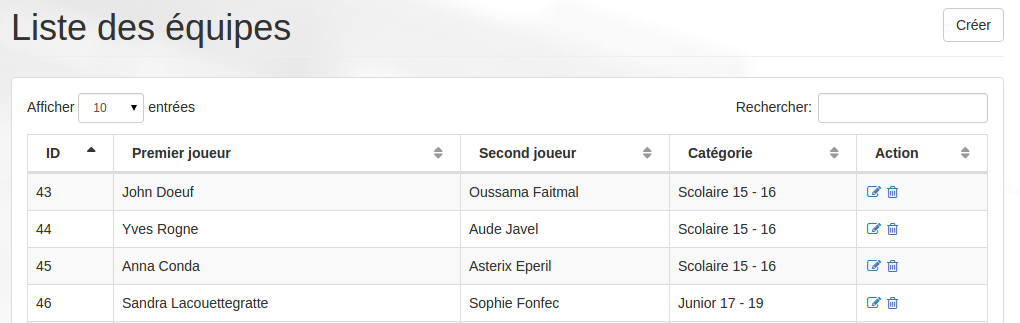
\includegraphics[scale=0.7]{tableau.png}
\caption{Example of a displayed table of list.php}
\end{figure}

\begin{figure}[H]
\centering
\includegraphics[scale=0.7]{show.png}
\caption{Example of displayed detail of an entity}
\end{figure}

\begin{figure}[H]
\centering

\includegraphics[scale=0.7]{form.png}
\caption{Example of a addition view (player.php, owner.php...)}
\end{figure}

And you will find bellow the name of files relating to the addition, edition and display of the different entities (table \ref{fig:staffpages}):

\fbox{Variables globales ?}

\begin{figure}[H]
\begin{center}
\begin{tabular}{|c|c|c|c|}
\hline
 Entity & Add & Edit & Show\\
 \hline
 \multirow{2}{*}{Pair/Player} & \multirow{2}{*}{player.php} & \multirow{2}{*}{edit-player.php} & list.php?type=player \\
  & & & show.php?type=player\\
\hline
 \multirow{2}{*}{Team} & \multirow{2}{*}{team.php} & \multirow{2}{*}{edit-team.php} & list-team.php\\
  & & & show-team.php\\
 \hline
 \multirow{2}{*}{Match} & \multirow{2}{*}{match.php} & \multirow{2}{*}{edit-match.php} & list-match.php\\
  & & & show-match.php\\
 \hline
 \multirow{2}{*}{Category} & \multirow{2}{*}{category.php} & \multirow{2}{*}{edit-category.php} & list.php?type=category \\
  & & & show.php?type=category\\
 \hline
 \multirow{2}{*}{Owner} & \multirow{2}{*}{owner.php} & \multirow{2}{*}{edit-owner.php} & list.php?type=owner \\
  & & & show.php?type=owner\\
 \hline
 \multirow{2}{*}{Court} & \multirow{2}{*}{court.php} & \multirow{2}{*}{edit-court.php} & list.php?type=court \\
  & & & show.php?type=court\\
 \hline
 \multirow{2}{*}{Extra} & \multirow{2}{*}{extra.php} & \multirow{2}{*}{edit-extra.php} & list-extras.php \\
  & & & show.php?type=extra\\
  \hline
 \multirow{2}{*}{Staff} & \multirow{2}{*}{-} & \multirow{2}{*}{-} & list.php?type=staff \\
  & & & show.php?type=staff\\
 \hline
 Groups & group-generate.php & group.php & group-overview.php \\
 \hline
 Knock-off & knock-off-generate.php & knock-off.php & knock-off-results.php \\
 \hline
\end{tabular}
\end{center}
 \caption{Name of the differents files of the folder \textit{src/staff/pages}}
 \label{fig:staffpages}
\end{figure}



\subsubsection{Modification of the database}
Every modifications of the database are done by the file of the folder \textit{src/staff/pages/php}.

\begin{figure}[H]
\centering
    \begin{tabular}{ccccc}
        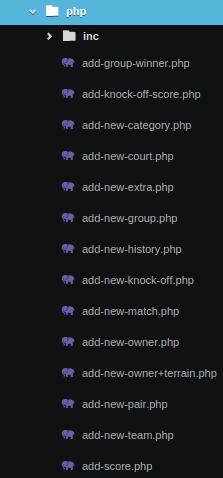
\includegraphics[scale=0.7]{arboAdd.png}
    &  &
        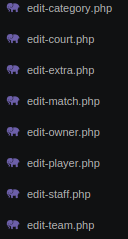
\includegraphics[scale=0.7]{arboEdit.png}
    &  &
        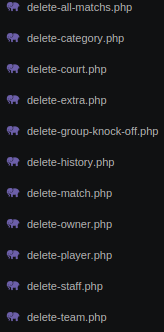
\includegraphics[scale=0.7]{arboDelete.png}
    \\
    \end{tabular}
\caption{Files which interact (add, edit, suppress) with the database}
\label{fig:maze}
\end{figure}

In the tabular \ref{fig:staffpagesphp}, we can see the names of the different files that can found in \textit{src/staff/pages/php}.
\begin{figure}[H]
\begin{center}
\begin{tabular}{|c|c|c|}
\hline
 Entity &  Add & Delete\\ \hline
 Pair/Player & add-new-pair.php &  delete-player.php \\
 Team & add-new-team.php &  delete-team.php \\
 Match & add-new-match.php &  delete-match.php \\
 Category & add-new-category.php & delete-category.php \\
 Owner & add-new-owner.php &  delete-owner.php \\
 Court & add-new-court.php &  delete-court.php\\
 Extra & add-new-extra.php &  delete-extra.php\\
 Staff & - & - \\
 \multirow{2}{*}{Groups} & add-new-group.php & \multirow{2}{*}{delete-group.php} \\
  & add-all-group.php & \\
 \multirow{2}{*}{Knock-off} & add-new-knock-off.php & \multirow{2}{*}{delete-knock.php} \\
  & add-all-knock-off.php & \\
 \hline
\end{tabular}
\end{center}
 \caption{Name of the different files of the folder \textit{src/staff/pages/php}}
 \label{fig:staffpagesphp}
\end{figure}

\subsubsection{Fichiers .inc}
The files .inc are in the folder \textit{src/staff/pages/php/inc} and contain every function in order to minimise the code in the other files.

\begin{figure}[H]
\centering
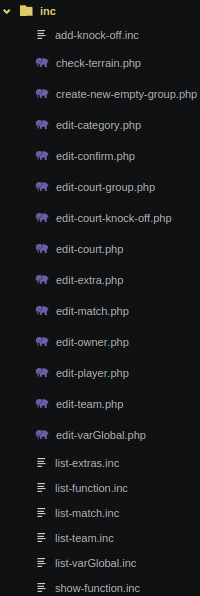
\includegraphics[scale=0.7]{arboInc.png}
\caption{}
\end{figure}

\subsection{Groups}
The groups management is split in five operations, which include the generation of the groups and their modification by the staff once they have been automatically generated. Then, there is the part where the staff can enter the scores and choose the victors. \\

Finally, there is the display of the groups, which is essentially working like any other listing page (like list.php).

Like usual, every pages required for this part can be found in
src/staff/pages(/php/inc).

\subsubsection{Generate}
First of all, the groups needs to be generated. There is two way for the staff to do this: generate the groups for a selected day and category (in \textit{./php/add-new-group.php}), or generate every groups for a selected day (in \textit{./php/add-all-groups.php}).

\subsubsection{Modify}
Once the groups are generated, the staff can still modify it to make sure that every team's wishes are satisfied. We implemented this part in the file \textit{src/staff/pages/group.php}. This pages is one of the most complicated of the website, because it holds a lot of functionalities. Follows the list of the files related to each one of these functionalities:
\begin{itemize}
\item Send a mail to the leader of a group: \textit{./mailLeader.php};
\item Send a mail to the players of the group that has not paid yet: \textit{./mailNP.php};
\item Send a mail to every member of a group: \textit{./mailAll.php};
\item Switch two teams between groups: \textit{./php/group-switch.php};
\item Show the wishes (might be empty) of a team: \textit{./php/group-note(-vide).php};
\item Change the leading team of a group: \textit{./php/promote-group-leader.php};
\item Delete one of the group: \textit{./php/delete-group.php};
\item Get the pdf format of a group: \textit{./php/print-group.php};
\item Check that every court for every group is different for a given day: \textit{./php/inc/check-terrain.php};
\item Create a new empty group: \textit{./php/inc/create-new-empty-group.php};
\item Change the court assigned to a group: \textit{./php/inc/edit-court-group.php};
\end{itemize}

\begin{figure}[H]
\centering
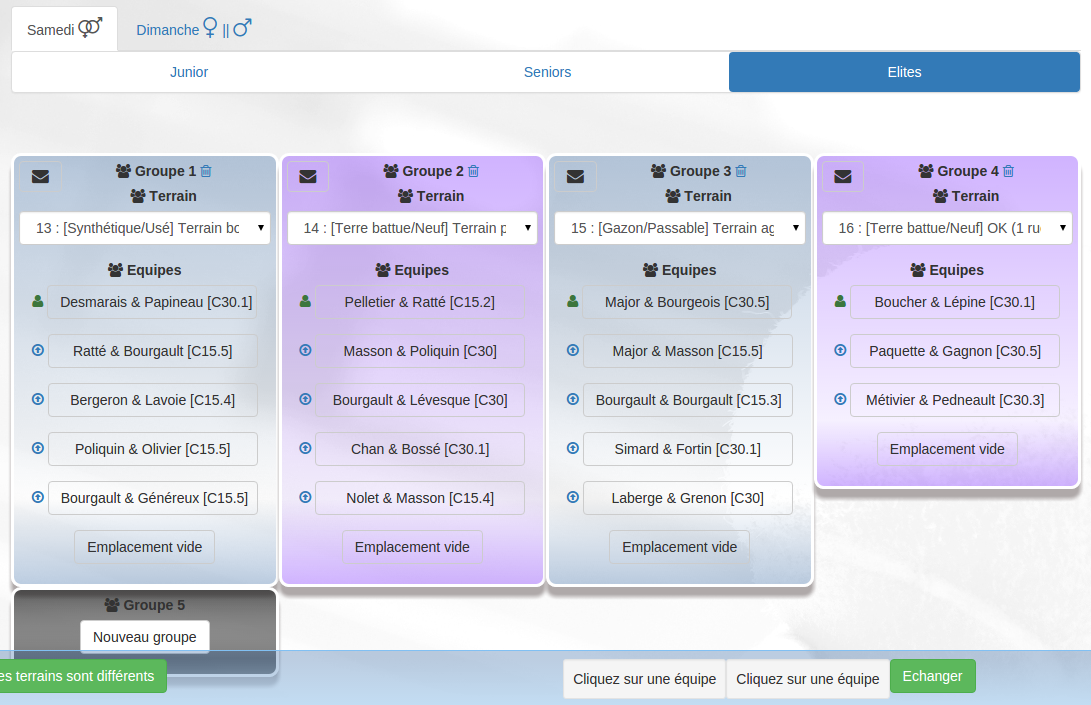
\includegraphics[scale=0.5]{group.png}
\caption{The modification page for the groups}
\end{figure}

\subsubsection{Input the scores}
After the groups have been reorganized by the staff, printed, and played by the teams, the staff needs to input the scores of the played matches. This is done on the page \textit{./input-group-score.php}. This page calls to two other pages, which are \textit{./php/add-group-score.php} and \textit{./php/modify\_global\_var.php}. Those pages are respectively for memorizing the inputted scores and modify the global variable \textit{tournament\_started} of the selected day, so that the groups can't be modified afterward.

\subsubsection{Input the victors}
When doing the previous part of the job, inputting the scores, the victors of the groups are automatically selected: if a team has won more than half its matches, it is considered a victor. This is a dynamic way of selecting the winning teams, but is not sufficient by itself, as the staff wants to be able to choose entirely who is qualified or not for the next part of the tournament. They can do this when selecting the victors, on the page \textit{./group-winner.php}, which calls \textit{./php/add-group-winner.php} to interact with the database.


\subsection{Knock-off}
As for the groups, the management of the knock-off tournament is split in several pages, each corresponding to a step in the tournament: the generation, the modification and check by the staff, and finally inputting the scores. Of course, there is always the display of the results, done on \textit{src/staff/pages/knock-off-results.php}.

\subsubsection{Generate}
Like for the groups, the knock-off can be generated (on \textit{./knock-off-generate.php}) for a single category, or for all of them, respectively done in \textit{./php/add-new-knock-off.php} and \textit{./php/add-all-knock-off.php}. Both of these pages call for a generic function that can be found in \textit{./php/inc/add-knock-off.inc}. This function create a single knock-off, given a category.

\subsubsection{Modify}
When coming to modify the automatically generated knock-off (on page \textit{./knock-off.php}), the functionalities available are very similar to those found on the group modifying page.

\begin{itemize}
\item Get the pdf format of the tournament: \textit{./php/print-knock-off.php}
\item Switch two teams between matches: \textit{./php/knock-off-switch.php}
\item Show the wishes of a team: \textit{./php/knock-off-note.php}
\item Show the wishes of a team when there is none: \textit{./php/groupe-note-vide.php}
\item Change the court assigned to a match: \textit{./php/inc/edit-court-knock-off.php}
\item Check that every court for every match of the first round is different for a given day: \textit{./php/inc/check-terrain.php}
\end{itemize}


\subsubsection{Input the scores}
And finally, the scores can be entered by the staff on the page \textit{./input-knock-score.php}. Three different pages are used by this functionality:

\begin{itemize}
\item To select a team that has won, making it pass to the next round: \textit{./php/select-team-knock-off.php}
\item When wanting to undo the selection of a team we just made: \textit{./php/delete-knock.php}
\item The function that dynamically update the scores entered by the staff: \textit{./php/add-score-knock-off.php}
\end{itemize}

\begin{figure}[H]
\centering
\includegraphics[scale=0.7]{knockoff-score.png}
\caption{The score input for the knock-off}
\end{figure}

\subsection{Confirmation d'inscription}
\fbox{on le met où?}

\section{Structure de la Base de données}
La Base de données utilisées est en MySQL

\begin{figure}[H]
\centering
\includegraphics[scale=0.7]{diagramme.png}
\caption{}
\end{figure}

\begin{figure}[H]
\centering
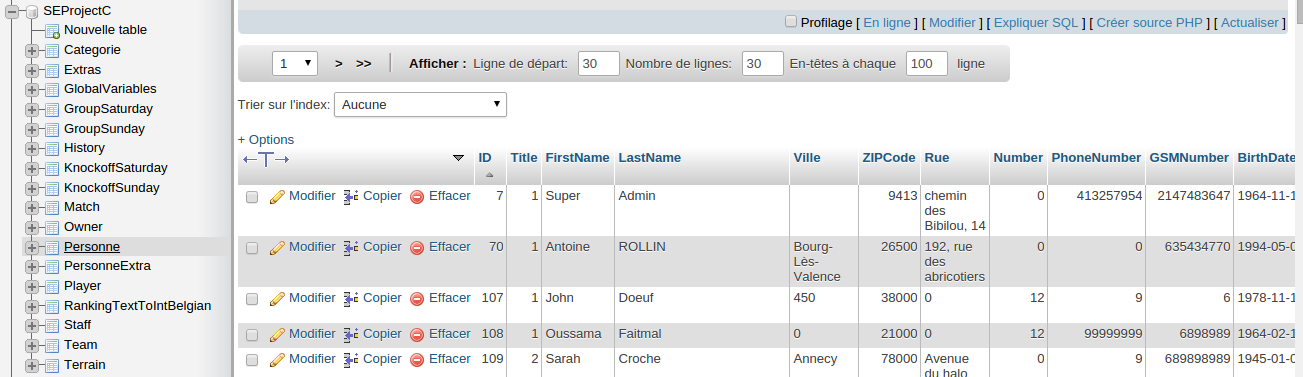
\includegraphics[scale=0.7]{phpMyAdmin.png}
\caption{}
\end{figure}

La  base  de  données  est  de  type SQL. Elle  correspond  au  fichier  de  format  ‘.sql’  dans  le dossier ‘docs’.

La  base  de  données  contient  les  différentes  tables  nécessaires  au  fonctionnement  de l’application :

\begin{itemize}
\item[$\bullet$]{\textbf{Categorie :}} contain the differents categories possible (a category is assigned to a team according to the age of the older member between the two players)

\item[$\bullet$]{\textbf{Extras :}} contain the extras, i.e the additionals activities proposed to the players.

\item[$\bullet$]{\textbf{GlobalVariables :}} contain diverse global variable like general message to send by mail, price of tournament, and know if the tournament has begun.

\item[$\bullet$]{\textbf{GroupSaturday :}} contain the groups of saturday's tournament.

\item[$\bullet$]{\textbf{GroupSunday :}} contain the groups of sunday's tournament

\item[$\bullet$]{\textbf{History  :}}  contain the history of modification. The history is update when a member of the staff add, suppress or edit a content.

\item[$\bullet$]{\textbf{KnockoffSaturday :}} contain the knock-off of saturday's tournament
contient tous les matchs de Knock-Off du samedi (liée à la table Match)

\item[$\bullet$]{\textbf{KnockoffSunday  :}}  contain the knock-off of sunday's tournament  (linked to the Match table)

\item[$\bullet$]{\textbf{Match :}} contain all matches of the tournament

\item[$\bullet$]{\textbf{Owner :}} contain all the informations relating to the owners registered (linked to the Personne table)

\item[$\bullet$]{\textbf{Personne  :}}  contain every personal informations of person registered (player, owner and staff)

\item[$\bullet$]{\textbf{PersonneExtra :}} contain the extra choice of players (linked to the Personne table)

\item[$\bullet$]{\textbf{Player :}} contain the informations of person registered as a player

\item[$\bullet$]{\textbf{RankingTextToIntBelgian :}} contain all official ranking possible

\item[$\bullet$]{\textbf{Staff  :}} contain all information relating to the staff members (linked to the Personne table)

\item[$\bullet$]{\textbf{Team :}} contain every team registered

\item[$\bullet$]{\textbf{Terrain :}} contain registered court which will be used for the tournament (linked to the Owner table)

\item[$\bullet$]{\textbf{PlayerAlone :}} contain player who don't have a team

\item[$\bullet$]{\textbf{OldOwner :}} contain the owner registered previous years

\item[$\bullet$]{\textbf{OldCourt :}} contain the court registered previous years

\item[$\bullet$]{\textbf{TmpPersonne :}} contain every personal informations of person who don't have confirm their registration with the verification mail

\item[$\bullet$]{\textbf{TmpPersonneExtra :}} contain the extra choice of players who don't have confirm their registration with the verification mail

\item[$\bullet$]{\textbf{TmpPlayer :}} contain the informations of person as player who don't have confirm their registration with the verification mail

\item[$\bullet$]{\textbf{TmpTeam :}} contain every team of players who don't have confirm both their registration
\end{itemize}


\section{Test}
\subsection{Ghost Inspector}

Logiciel payant limité à 100 test par mois. Facilité de générer des scripts\\
\begin{figure}[H]
\centering
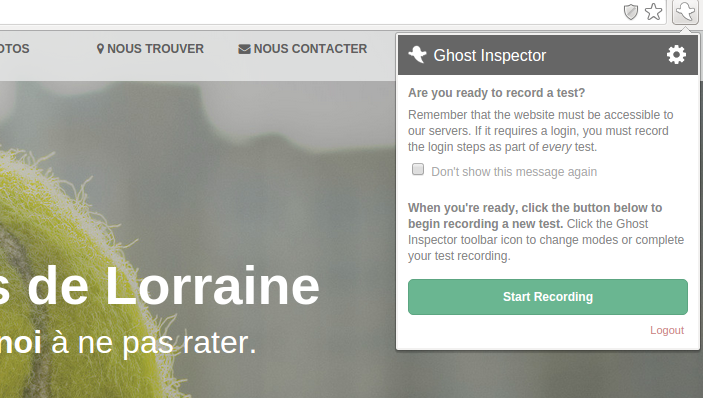
\includegraphics[scale=0.7]{ghost.png}
\caption{Démarrer une simulation}
\end{figure}

\begin{figure}[H]
\centering
\includegraphics[scale=0.7]{ghostInterface.png}
\caption{Gérer ses tests}
\end{figure}

\subsection{Selenium}

Executer un script\\
\begin{figure}[H]
\centering
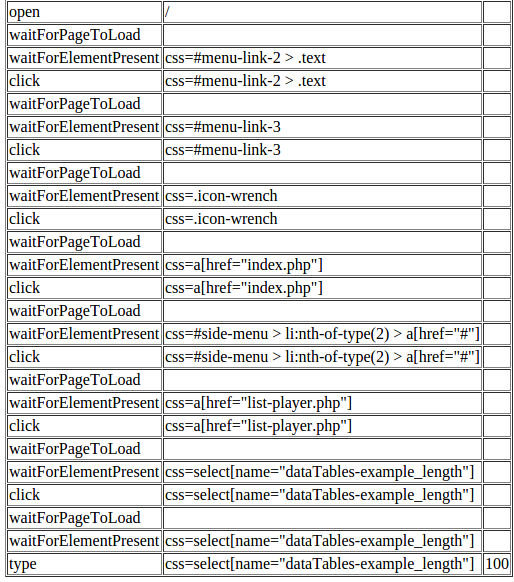
\includegraphics[scale=0.7]{selenium.png}
\caption{}
\end{figure}

\section{Conclusion}
``I always thought something was fundamentally wrong with the universe'' \citep{adams1995hitchhiker}

\bibliographystyle{plain}
\bibliography{references}

\end{document}
